\documentclass[tikz,border=5mm]{standalone}
\usepackage[utf8]{vietnam}
\usetikzlibrary{calc,angles,patterns,quotes,intersections}

\begin{document}
	
	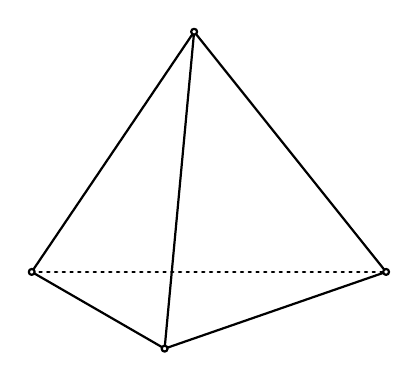
\begin{tikzpicture}[join=round,cap=round,thick,scale=.75]
		\def\a{3}
		\pgfmathsetmacro\b{\a *cos(60)}
		\path
		(180:\a)  coordinate (A)
		(-120:\b) coordinate (C)
		(0:\a)coordinate (B)
		($(B)!.5!(C)$) coordinate (M)
		($(A)!.5!(C)$) coordinate (N)
		(intersection of A--M and B--N) coordinate (O)
		(O)+(90:1.5*\a) coordinate (S)
		;
		\draw[dotted] (A)--(B);
		\draw (A)--(C)--(B)--(S)--cycle (S)--(C);
		\foreach \x in {A,B,C,S} \draw[fill=white](\x) circle (.05);
	\end{tikzpicture}
	
	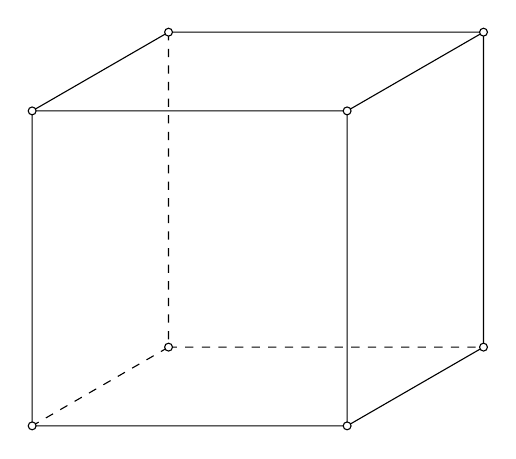
\begin{tikzpicture}
		\def\a{4}
		\path
		(0:0) coordinate (A)
		(0:\a) coordinate (B)
		++(30:\a/2) coordinate (C)
		++(180:\a) coordinate (D)
		\foreach \x in {A,B,C,D}{(\x)++(90:\a) coordinate (\x_1)}
		;
		\draw[dashed] (D_1)--(D)--(A) (D)--(C);
		\draw
		(A)--(B)--(C) (A)--(A_1) (B)--(B_1) (C)--(C_1)
		(A_1)--(B_1)--(C_1)--(D_1)--cycle
		;
		\foreach \x in {A,B,C,D,A_1,B_1,C_1,D_1} \draw[fill=white] (\x) circle (.05);;
	\end{tikzpicture}
	
	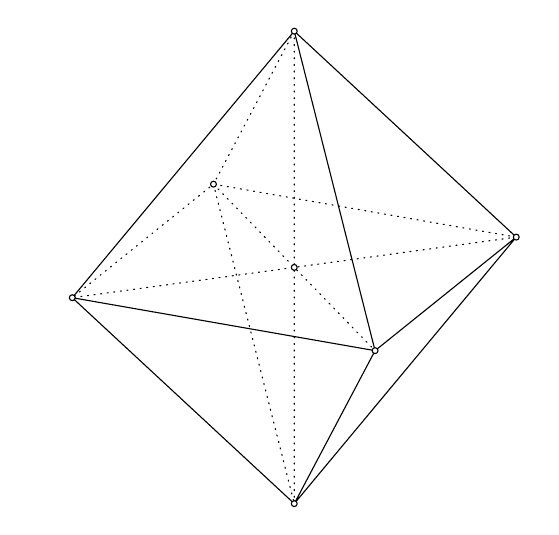
\begin{tikzpicture}[join=round,cap=round,scale=.75]
		\def\a{4}
		\def\b{1.5}
		\def\gA{20}
		\path
		(0:0) coordinate (O)
		(0:\a) arc (0:\gA:{\a} and {\b}) coordinate (A)
		arc (\gA:\gA+90:{\a} and {\b}) coordinate (B)
		arc (\gA+90:\gA+180:{\a} and {\b}) coordinate (C)
		arc (\gA+180:\gA+270:{\a} and {\b}) coordinate (D)
		(O)+(90:\a) coordinate (E)
		(O)+(-90:\a) coordinate (F)
		;
		\draw[dotted]
		(E)--(F) (A)--(C) (B)--(D)
		(A)--(B)--(C) (E)--(B)--(F)
		;
		\draw
		(E)--(A)--(F) (E)--(C)--(F) (E)--(D)--(F)
		(C)--(D)--(A)
		;
		\foreach \x in {A,B,C,D,O,E,F} \draw[fill=white](\x) circle (.05);
	\end{tikzpicture}
	
	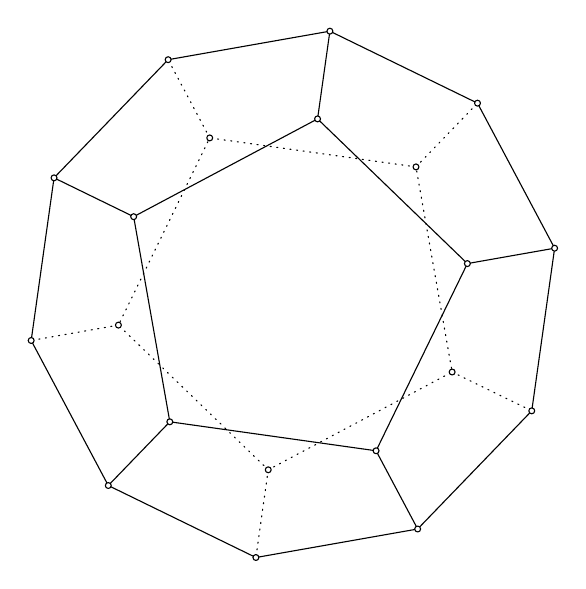
\begin{tikzpicture}[join=round,cap=round,scale=.75]
		\def\r{3}
		\def\gA{10}
		\path
		(\gA:\r) coordinate (A_1)
		(\gA+72:\r) coordinate (A_2)
		(\gA+144:\r) coordinate (A_3)
		(\gA+216:\r) coordinate (A_4)
		(\gA+288:\r) coordinate (A_5)
		(\gA+36:\r) coordinate (B_1)
		(\gA+108:\r) coordinate (B_2)
		(\gA+180:\r) coordinate (B_3)
		(\gA+252:\r) coordinate (B_4)
		(\gA+324:\r) coordinate (B_5)
		\foreach \i in {1,...,10}{(\gA+\i *36-36:1.5*\r) coordinate (C_\i)}
		;
		\draw[dotted]
		(B_1)--(B_2) --(B_3)--(B_4)--(B_5)--cycle
		(B_1)--(C_2) (B_2)--(C_4) (B_3)--(C_6) (B_4)--(C_8) (B_5)--(C_10)
		;
		\draw
		(A_1)--(A_2)--(A_3)--(A_4)--(A_5)--cycle
		(A_1)--(C_1) (A_2)--(C_3) (A_3)--(C_5) (A_4)--(C_7) (A_5)--(C_9)
		(C_1)--(C_2)--(C_3)--(C_4)--(C_5)--(C_6)--(C_7)--(C_8) --(C_9)--(C_10)--cycle
		;
		\foreach \x in {A_1,A_2,A_3,A_4,A_5,B_1,B_2,B_3,B_4,B_5,C_1,C_2,C_3, C_4,C_5,C_6,C_7, C_8,C_9,C_10} \draw[fill=white] (\x) circle (.05);
	\end{tikzpicture}
	
	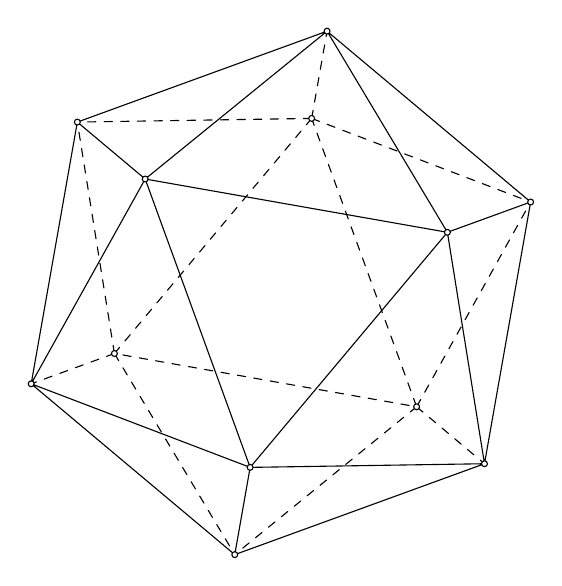
\begin{tikzpicture}[join=round,cap=round,scale=.75]
		\def\r{3}
		\def\gA{20}
		\path
		(\gA:\r) coordinate (A_1)
		(\gA+120:\r) coordinate (A_2)
		(\gA+240:\r) coordinate (A_3)
		(\gA+60:\r) coordinate (B_1)
		(\gA+180:\r) coordinate (B_2)
		(\gA+300:\r) coordinate (B_3)
		\foreach \i in {1,...,6}{(\gA+\i *60-60:1.5*\r) coordinate (C_\i)}
		;
		\draw[dashed] 
		(B_1)--(B_2)--(B_3)--cycle
		(B_1)--(C_1) (B_1)--(C_2) (B_1)--(C_3)
		(B_2)--(C_3) (B_2)--(C_4) (B_2)--(C_5)
		(B_3)--(C_5) (B_3)--(C_6) (B_3)--(C_1)
		;
		\draw
		(A_1)--(A_2)--(A_3)--cycle
		(A_1)--(C_6) (A_1)--(C_1) (A_1)--(C_2)
		(A_2)--(C_2) (A_2)--(C_3) (A_2)--(C_4)
		(A_3)--(C_4) (A_3)--(C_5) (A_3)--(C_6)
		(C_1)--(C_2) --(C_3)--(C_4)--(C_5)--(C_6)--cycle
		;
		\foreach \x in {A_1,A_2,A_3,B_1,B_2,B_3,C_1,C_2,C_3,C_4,C_5,C_6} \draw[fill=white] (\x) circle (.05);
	\end{tikzpicture}
\end{document}